\begin{verbatim}
from IPython.display import HTML
from IPython.display import Image


# from http://blog.nextgenetics.net/?e=102
HTML('''<script>
code_show=true; 
function code_toggle() {
 if (code_show){
 $('div.input').hide();
 } else {
 $('div.input').show();
 }
 code_show = !code_show
} 
$( document ).ready(code_toggle);
</script>
The raw code for this IPython notebook is by default hidden for easier reading.
To toggle on/off the raw code, click <a href="javascript:code_toggle()">here</a>.''')
\end{verbatim}

The raw code for this IPython notebook is by default hidden for easier
reading. To toggle on/off the raw code, click here.

\section{Open Data: The Why and How of Contributing to and Benefitting
from the Open Data
Ecosystem}\label{open-data-the-why-and-how-of-contributing-to-and-benefitting-from-the-open-data-ecosystem}

\begin{quote}
\emph{Karl Benedict} - Director of Research Data Services, College of
University Libraries and Learning Sciences

University of New Mexico

kbene@unm.edu
\end{quote}

\subsection{Presentation Outline}\label{presentation-outline}

\begin{center}\rule{0.5\linewidth}{\linethickness}\end{center}

\begin{itemize}
\itemsep1pt\parskip0pt\parsep0pt
\item
  Introduction
\item
  Current Context
\item
  A Quick Refresher on Geospatial Interoperability Standards
\item
  Where \& How You Can Get Stuff
\item
  Where Your Stuff Can Go
\end{itemize}

\begin{center}\rule{0.5\linewidth}{\linethickness}\end{center}

\subsection{Introduction}\label{introduction}

\begin{center}\rule{0.5\linewidth}{\linethickness}\end{center}

\begin{itemize}
\itemsep1pt\parskip0pt\parsep0pt
\item
  The Geospatial Community Has a Long Tradition of Open Data \& Data
  Sharing
\end{itemize}

\begin{figure}[htbp]
\centering

\includegraphics{images/NMRGIS_Logo.png}
\caption{NM RGIS Logo}
\end{figure}

\begin{center}\rule{0.5\linewidth}{\linethickness}\end{center}

\begin{figure}[htbp]
\centering
\includegraphics{images/The_Federal_Geographic_Data_Committee_—_Federal_Geographic_Data_Committee.png}
\caption{FGDC}
\end{figure}

\begin{center}\rule{0.5\linewidth}{\linethickness}\end{center}

\begin{figure}[htbp]
\centering

\includegraphics{images/geodata_gov.png}
\caption{Geospatial OneStop}
\end{figure}

\begin{center}\rule{0.5\linewidth}{\linethickness}\end{center}

\begin{figure}[htbp]
\centering
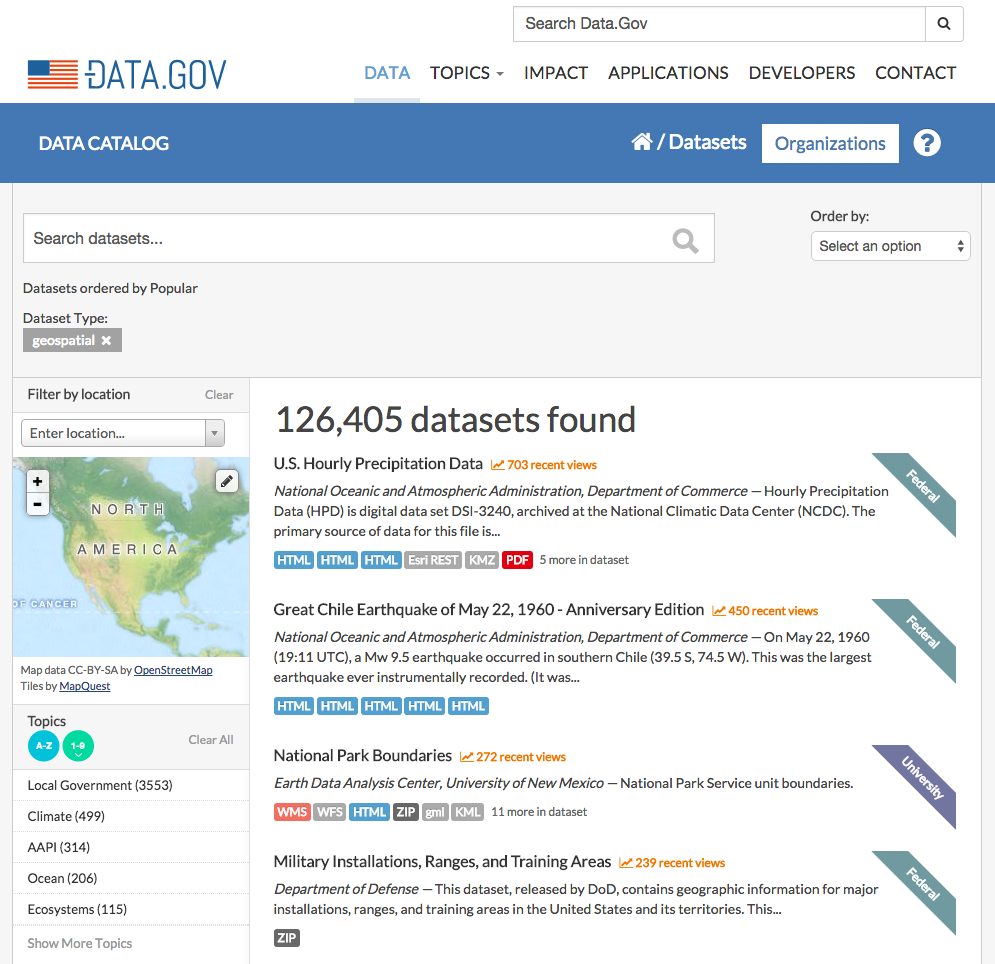
\includegraphics{images/Search_for_a_Dataset_-_Data_gov.png}
\caption{Catalog.data.gov}
\end{figure}

\begin{center}\rule{0.5\linewidth}{\linethickness}\end{center}

\begin{itemize}
\itemsep1pt\parskip0pt\parsep0pt
\item
  Open standards to support geospatial data discovery, visualization and
  access
\end{itemize}

\begin{center}\rule{0.5\linewidth}{\linethickness}\end{center}

\includegraphics{images/The_Federal_Geographic_Data_Committee_—_Federal_Geographic_Data_Committee.png}
- FGDC Content Standard for Digital Geospatial Metadata

\begin{center}\rule{0.5\linewidth}{\linethickness}\end{center}


\includegraphics{images/ISO_-_International_Organization_for_Standardization.png}
- ISO 19115/19115-2/19115-1 and related standards

\begin{center}\rule{0.5\linewidth}{\linethickness}\end{center}


\includegraphics{images/OGC_Logo_2D_Blue_x_0_0.png} - Open Geospatial
Consortium

\subsection{Current Context}\label{current-context}

\begin{center}\rule{0.5\linewidth}{\linethickness}\end{center}

\begin{center}\rule{0.5\linewidth}{\linethickness}\end{center}

\subsection{A Quick Refresher on Geospatial Interoperability
Standards}\label{a-quick-refresher-on-geospatial-interoperability-standards}

\begin{center}\rule{0.5\linewidth}{\linethickness}\end{center}

\begin{center}\rule{0.5\linewidth}{\linethickness}\end{center}
